\documentclass[10pt,twocolumn,letterpaper]{article}

\usepackage{cvpr}
\usepackage{times}
\usepackage{epsfig}
\usepackage{graphicx}
\usepackage{amsmath}
\usepackage{amssymb}
\usepackage[pagebackref=true,breaklinks=true,letterpaper=true,colorlinks,bookmarks=false]{hyperref}
\def\cvprPaperID{****} % *** Enter the CVPR Paper ID here
\def\httilde{\mbox{\tt\raisebox{-.5ex}{\symbol{126}}}}
\ifcvprfinal\pagestyle{empty}\fi
\begin{document}

%%%%%%%%% TITLE
\title{DRAGN: Deep Recusively AggreGation Network}

\author{First Author\\
Institution1\\
Institution1 address\\
{\tt\small firstauthor@i1.org}
\and
Second Author\\
Institution2\\
First line of institution2 address\\
{\tt\small secondauthor@i2.org}
}

\maketitle

%%%%%%%%%%%%%%%%%%%%%%%%%%% ABSTRACT %%%%%%%%%%%%%%%%%%%%%%%%%%%%%%%%%%%%
\begin{abstract}
A lot of computer vision tasks exhibit multi-instance property, in which the learning is performed at the bag-level instead of instance-level and each bag contains of multiple instances, i.e. images. Compared to traditional multi-instance learning algorithms and recent 3D deep neural networks, feature aggregation methods have the following advantages: i)more flexible, as it can be achieved in both traditional and deep learning frameworks, and ii)more versatile, as it can deal with various types of bags without temporal or spatial dependency between images.

In this study, we proposed a deep learning-based feature aggregation model, called DRAGN(Deep Recursively AggreGation Network). It consists of two components, feature aggregation unit and feature aggregation module. The feature aggregation module uses feature aggregation unit to perform iterative and stacked convolution aggregation of multiple instances, and finally output an aggregated feature.

We assess the model performance on two biomedical image processing tasks. One is the protein subcellular localization using immunofluorescence images for human cells, and the other is gene annotation using spatial gene expression images. In both the two tasks, DRAGN outperforms the existing feature aggregation methods and the state-of-the-art models for addressing these two tasks.

\end{abstract}

%%%%%%%%%%%%%%%%%%%%%%%%%%%%%%%%%% 1,introduction %%%%%%%%%%%%%%%%%%%%%%%%%%%%%%%%%%%%
\section{Introduction}

In traditional computer vision tasks, like image classification \cite{ref1, ref2, ref3}, object detection \cite{ref4, ref5}, and semantic segmentation \cite{ref6, ref7}, the inputs of computational learning models are single images. As image processing techniques develop rapidly and the storage capacity for multi-media data grows dramatically, there is an increasing need for handling higher dimensional data, including videos, series of images, ect. Especially, in many image processing applications, the input consists of multiple images, which determine the output jointly. For example, when we recognize person identity based on videos, each video input can be regarded as a time-series of images. Another example is the automatic diagnosis system based on MRI (magnetic resonance imaging) data, which consists of multiple slices presenting the area of interest being scanned. In these two cases, there are either temporal or spatial dependency between images; whereas for a lot more applications, their inputs are neither videos nor 3D models, but just bags of images. There may be no defined spatio-temporal relationship between images, but they have common attributes associated with the bag. For instance, in a video surveillance task, we use multiple cameras to take photos of the same person at multiple time slots and locations. Apparently, these photos, with different lighting conditions and backgrounds, describe the same person. 

% 第一个图
\begin{figure}[t]
\begin{center}
% \fbox{\rule{0pt}{2in} \rule{0.9\linewidth}{0pt}}
  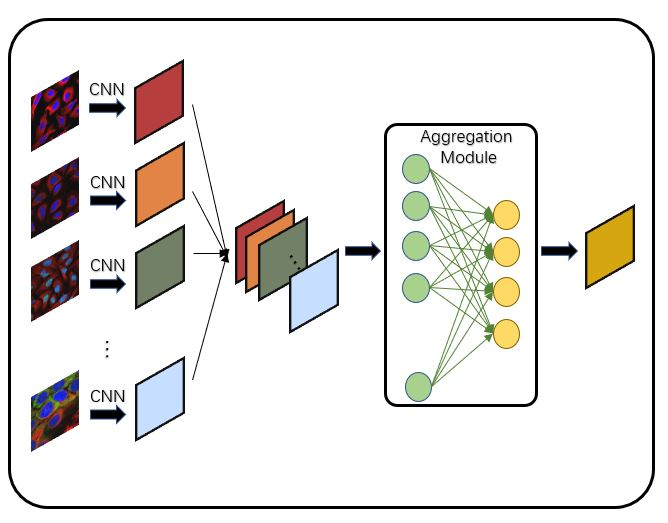
\includegraphics[width=0.8\linewidth]{figure1.JPG}
\end{center}
   \caption{A simple schematic of feature aggregation,The pretrained CNN model is used to extract features from the input images, and then the extracted features are input into the feature aggregation module to obtain the final aggregation output. }
\label{fig:long}
\label{fig:onecol}
\end{figure}

Such multi-image-input (MII) tasks are especially common in the biomedical field. 
Benefitting from recent advances of microscopic imaging technology, various types of biomedical images have accumulated at an unprecedented rate for the past decade \cite{ref11,ref12,ref13,ref14}. Image analysis has become a common approach in not only medical diagnosis but also fundamental biological researches from tissue level down to the cell level. 

Unlike natural images, biomedical images are often much harder to obtain due to the difficulty in preparing the specimen or stringent experimental conditions. Therefore, during the imaging procedure, it is common to capture multiple images for a specimen in a single trial of experiment and perform multiple trails for repeatability. To infer the functions of genes or characteristic of molecules, all the captured images should be considered comprehensively to give a more accurate judgement on the final output, as single images may only contain partial information and it is important to capture the correlation between images. 

For the MII tasks, there are two major computational challenges.
\begin{itemize}
\item i) Variable input bag size. In MII tasks, the number of input images is usually nonfixed, especially when the bags differ greatly in their sizes, which adds difficulty to machine learning models.
\item ii) Uneven quality of images. Usually, high-quality images and uninformative images are mixed together in the same bag. Thus, how to make the model focus on important images and ignore irrelevant information is a key issue in MII tasks.
\end{itemize}

To address MII learning tasks, there are 3 possible solutions.


i) \textbf{Multi-instance learning (MIL) models.}
The MII learning tasks can be regarded as a special kind of problems in machine learning, namely multi-instance learning. As MIL is a general learning framework, it can deal with any type of multi-instance input, including image, text, chemical structures, etc. MIL algorithms compute pair-wise similarity or loss function at the bag-level instead of instance-level. Till now, a lot of MIL methods have been developed, like multi-instance KNN and multi-instance SVM. Before using these traditional learning models, image features should be extracted separately. Recently, a deep-learning-based MIL model has been proposed, called DeepMIML \cite{Feng2017AAAI}, but it was designed for single-image input and each image is regarded as a bag of objects. 

  
ii) \textbf{Feature aggregation methods.}
Instead of adapting learning models to multi-instance inputs, this type of methods focuses on feature representations. There are a few ways to combine instance-level features to bag-level representation. For instance, in image retrieval, researchers aggregated the patch-based local descriptors into a global descriptor \cite{bov, perronnin2010improving, arandjelovic2013all}. Moreover, deep learning models can conveniently achieve feature aggregation by simply using pooling, summation or averaging operations. Some state-of-the-art models are introduced in details in Section \ref{sec:related}.

iii) \textbf{Models with direct 3D input}
Recent advances of deep learning methods allow a more straightforward processing of high-dimensional data. Instead of regarding the input as a bag of images, we can feed the 3D data structure directly into a 3D CNN. 


Apparently, the third type of methods is more suitable for processing video data or 3D models, in which the images have strong correlations with each other. The first type of methods are mostly traditional shallow learning models. For dealing with image data, extra feature engineering is required. By contrast, the second type is more versatile, including both traditional and deep learning-based models, and can be applied to learn representations for various bags of images.

In this paper, we focus on feature aggregation, because of its flexibility in dealing with various types of image sets, especially originated from biomedical studies, and propose a model, called DRAGN (Deep Recusively AggreGation Network). The main contributions of this paper are as follows:

First of all, this paper proposes a general framework for feature aggregation of multi-input single-output design pattern models. This framework has two variants,pre-aggregation and post-aggregation, both of which can effectively conduct feature aggregation.

Secondly, this paper proposes a new feature aggregation module, which includes network complexity optional feature aggregation units and a new feature aggregation process. The feature aggregation module can handle multiple input samples with different length, so that the network is no longer limited by the fixed input samples number.

Finally, we conducted experiments on the human protein atlas data set and the flyexpress data set, and we compared the experimental results with other relevant studies. The experimental results proved that our feature aggregation module has quite obvious advantages in improving the performance of the downstream tasks.

%%%%%%%%%%%%%%%%%%%%%%%%%%%% 2, relate work %%%%%%%%%%%%%%%%%%%%%%%%%%%%%%%%%%%%
\section{Relate Work}
Feature aggregation is fairly common in the field of computer vision. In video monitoring and face recognition tasks, if multiple photos of the same person taken by different cameras can be sent to the network model for training at the same time, the generalization ability of the model will be greatly enhanced and the accuracy of model recognition will be improved. This will make it easier for the network to grasp the correlation between different images of the same person than send single image to the network for training, while, this correlation information is the key factor for the network to make a right judgement.

%%%%%%%%% 第二个模块大图 %%%%%%%%%%%%%%%%%%%%%%%%%%%
\begin{figure*}
\begin{center}
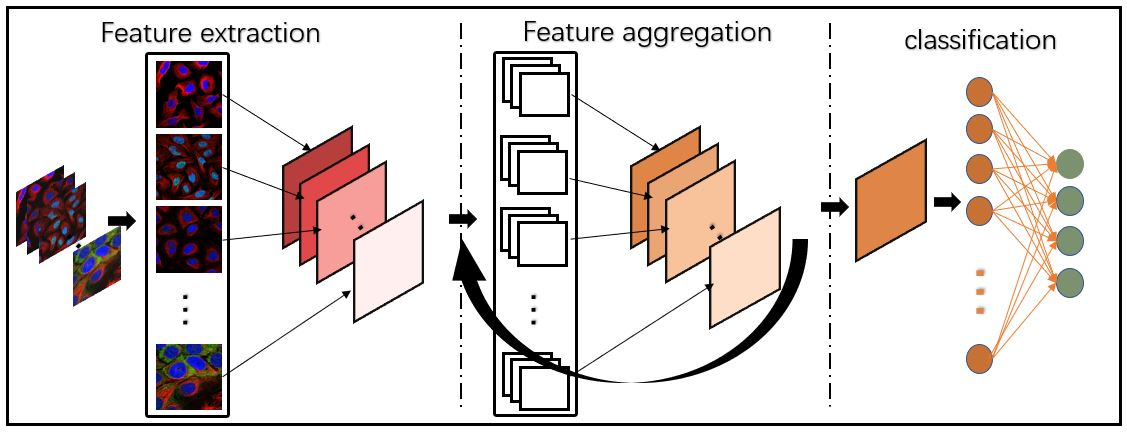
\includegraphics[width=0.8\linewidth]{framework.JPG}
\end{center}
   \caption{The main model framework for the DRAGN that we proposed in our paper.}
\label{fig:short}
\end{figure*}

\textbf{Traditional methods} 
In traditional image processing, feature aggregation is a part of feature engineering, which aims to fuse features extracted from single images into a comprehensive feature representation and feed to a learning model. There are three typical feature fusion methods, namely the bag of visual words (BOV) \cite{bov}, Fisher vector \cite{fishervector}, and vector of locally aggregated descriptors (VLAD) \cite{vlad}. BOV regards image features as words, builds a vocabulary of local image features and generates a vector of their occurrence counts. The Fisher vector method stores the mixing coefficients of the Gaussian mixture model (GMM) as well as the mean and covariance deviation vectors of the individual components. The VLAD method computes the distance of each feature point to the cluster center closest to it. All of these three methods produce a fixed-length feature vector for the input image set, which can work with traditional machine learning models, like support vector machines (SVMs).

\textbf{Deep learning-based methods} For the past decade, feature encoding via deep neural networks has almost replaced traditional feature engineering in image processing \cite{ref16, ref19, ref20}. Deep learning-based feature aggregation methods have also emerged. Actually, it is natural to fuse features by using the common operations, like pooling, summation or averaging in convolutional neural networks (CNNs). Su et al pioneered the studies that integrate feature aggregation into CNNs \cite{ref23}. To achieve 3D recognition by using photos captured from different angles, they designed a Multi-view CNN (MVCNN) model to extract photo features and fuse information from multiple orientations. The feature aggregation strategy in MVCNN is simply a maximization operation but very effective in the task. Later, Yang et al proposed a neural aggregation network for video face recognition, NAN\cite{ref24}, which exploited multiple face images to train the network model. Instead of a simple integration procedure, NAN aggregates multiple features by an attention module, which assigns high attention scores to important features.
Besides, by considering the feature vector of each instance as the input at a time step, Yang et al designed a model called Annofly \cite{annofly} based on recurrent neural network, which also implemented an attention mechanism to make the model focus on high-quality images.

In summary, these three methods aim to weight multiple input features by suitable weighting coefficients, so as to obtain final aggregated features, based on either CNN or RNN network architecture. The proposed DRAGN model also exploit the CNN model, but it integrates multiple input features into one feature through cyclic convolution.



In the next section, we will give a detailed introduction to our model.

%%%%%%%%%%%%%%%%%%%%%%%%%%%% 3, methods %%%%%%%%%%%%%%%%%%%%%%%%%%%%%%%%%%%%
%-------------------------------------------------------------------------
\section{Methods}
In this section, we will introduce in detail about the main framework of the model proposed in this paper and the main design mechanism for the feature aggregation.

%%%%%%%%%%% 3.1 Framework %%%%%%%%%%%
\subsection{Framework}
In this section, we will describe the overall framework of the model DRAGN in detail, which is shown in figure 2. In this paper, two schemes for feature aggregation, pre-aggregation and post-aggregation, are proposed.

%%%%%%%%%%% 3.1.1 post-aggregation %%%%%%%%%%%
\subsubsection{Post-aggregation}
The post-aggregation scheme mainly consists of two parts, namely feature extraction and feature aggregation, which are described below.

\textbf{Feature extraction}
We use the pre-trained CNN model to conduct feature extraction on the input images. The CNN model that can be selected includes resnet series, VGG series, Densenet, SENet, SEResnet, etc. In our paper, we chose the resnet series model. First, we will give the notation used in this paper, we donate the dataset as $\{x^{(i)}, y^{(i)}\}$, where i = $\{1,2,3,...,m\}$, m represents the number of training samples.Each $x^{(i)} = \{x^{(i)}_1, x^{(i)}_2, x^{(i)}_2,..., x^{(i)}_{n^{(i)}}\}$, where $n^{(i)}$ represents the number of multiple instances contained in the training sample. Because each training sample contains different number of multiple instances, the value of $n^{(i)}$ here will not be consistent. We donate the feature extraction function as $f_{ext}()$, and we donate the extracted feature as $o^{(i)}$, $o^{(i)} = \{o^{(i)}_1, o^{(i)}_2, o^{(i)}_3, ... ,o^{(i)}_{n^{(i)}}\}$, extraction process is as follows:
\begin{equation}
    o^{(i)}_j = f_{ext}(x^{(i)}_j)
\end{equation}
where $j = \{1,2,3,...,n^{(i)}\}$.

\textbf{Feature aggregation}
After the feature extraction in the previous step, we obtained the feature $o = \{o^{(1)}, o^{(2)}, o^{(3)}, ..., o^{(m)}\}$. In this step, feature aggregation is conducted to aggregate the feature of a multiple instance into the feature of a single instance. we donate the feature aggregation function as $f_{agg}()$, and the result after aggregation is denoted as $a_{(i)}$, each $a_{(i)}$ is obtaied by $o^{(i)}$ aggregation.The aggregation process is as follows:
\begin{equation}
    a^{(i)} = f_{agg}(o^{(i)}_1, o^{(i)}_2, ..., o^{(i)}_{n^{(i)}})
\end{equation}

%%%%%%%%%%% 3.1.2 pre-aggregation %%%%%%%%%%%
\subsubsection{Pre-aggregation}
Pre-aggregation and post-aggregation is basically the same, it is also formed by the feature extraction and feature aggregation. The main difference between them is that post-aggregation is to conduce feature extraction on the input and then conduct feature aggregation, while pre-aggregation is to conduct feature aggregation on the input and then conduct feature extraction.The operation process is as follows:

\textbf{Feature aggregation}
Using the same feature aggregation function as post-aggregation, the multiple input instances are aggregated into a single output instance as follows:
\begin{equation}
    o^{(i)} = f_{agg}(x^{(i)}_1, x^{(i)}_2, ..., x^{(i)}_{n^{(i)}})
\end{equation}

\textbf{Feature extraction}
After obtaining the aggregated input in the previous step, in this step, we used the pre-trained resnet model to conduct feature extraction:
\begin{equation}
    a^{(i)} = f_{ext}(o^{(i)})
\end{equation}

% 第三个图: L1Agg
\begin{figure}[t]
\begin{center}
% \fbox{\rule{0pt}{2in} \rule{0.9\linewidth}{0pt}}
  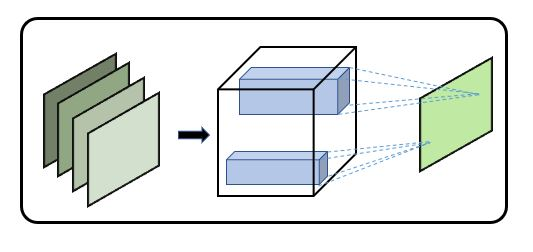
\includegraphics[width=0.8\linewidth]{figure4.JPG}
\end{center}
   \caption{Feature aggregation module: L1Agg module}
\label{fig:long}
\label{fig:onecol}
\end{figure}

%%%%%%%%%%% 3.1.3 Apply to downstream tasks %%%%%%%%%%%
\subsubsection{Apply to downstream tasks}
After feature extraction and feature aggregation, we get the final feature $a_{(i)}$, it can be applied to a variety of downstream tasks. In our case, our downstream task is classification, and we classify the final feature through a fully-connected layer. The fully-connected layer used for classification is denoted as $f_{fc}()$, and the prediction of classification is denoted as p, the prediction process is as follow:
\begin{equation}
    p_{(i)} = f_{fc}(a^{(i)})
\end{equation}

%%%%%%%%%%% 3.1.4 Loss Function %%%%%%%%%%%
\subsubsection{Loss Function}
We adopted various forms of loss functions, including the traditional classification loss function BCE, focal loss which is suitable for solving unbalanced multi-label classification task and FECLoss which is proposed in \cite{ref27}. When conducting experiments, we selectively use different loss functions on different datasets.

%%%%%%%%%%%%%%%%%%%%%% 3.2 Feature aggregation module %%%%%%%%%%%%%%%%%%%%
\subsection{Feature aggregation module}
In this section, we will introduce the design of DRAGN's feature aggregation module in detail, including the feature aggregation unit and the feature aggregation process.

%%%%%%%%%%% 3.2.1 Feature aggregation unit %%%%%%%%%%%
\subsubsection{Feature aggregation unit}
According to the requirement of different network complexity, we proposed three feature aggregation units, namely, L1Agg, L2Agg, L3Agg, among which the simplest is L1Agg, whose network model is shown in figure 3. As shown in the figure 3, it contains a convolution layer that receives the input of three features and gives an output feature after convolution. The next is L2Agg and L3Agg. Their network models are shown in figure 4, their netowrk models are respectively consist of conv + BN + relu + conv, and conv + BN + relu + conv + BN + relu + conv. As you can see, they are identical in usage, except for the complexity of the network model.

% 第四个图: L2Agg 和 L3Agg
\begin{figure}[t]
\begin{center}
% \fbox{\rule{0pt}{2in} \rule{0.9\linewidth}{0pt}}
  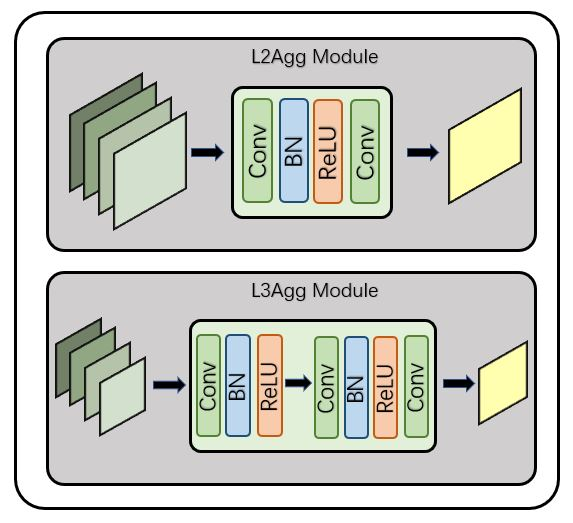
\includegraphics[width=0.8\linewidth]{figure5.JPG}
\end{center}
   \caption{Feature aggregation module: L2Agg module and L3Agg module }
\label{fig:long}
\label{fig:onecol}
\end{figure}


%%%%%%%%%%% 3.2.2 Feature aggregation process %%%%%%%%%%%
\subsubsection{Feature aggregation process}
After completing the design of feature aggregation units, in this step we will use these feature aggregation units to effectively aggregate the input features. The specific algorithm of feature aggregation process is shown in algorithm 1.

Assuming that there are n features in the input, in the first round of aggregation, we use the feature aggregation unit to select 3 features successively as the input to produce an aggregated output. After one round of aggregation, we will obtain n-2 aggregated feature. Then we will repeat the previous round, but this time we take the n-2 aggregated features from the previous round as the input and produce the new output. Repeat the aggregation process in turn, and finally we will obtain the final feature, when there are two features left after the last round of aggregation, we will take the mean value of them as the final feature.

% 第五个图: 特征融合过程算法
\begin{figure}[t]
\begin{center}
% \fbox{\rule{0pt}{2in} \rule{0.9\linewidth}{0pt}}
  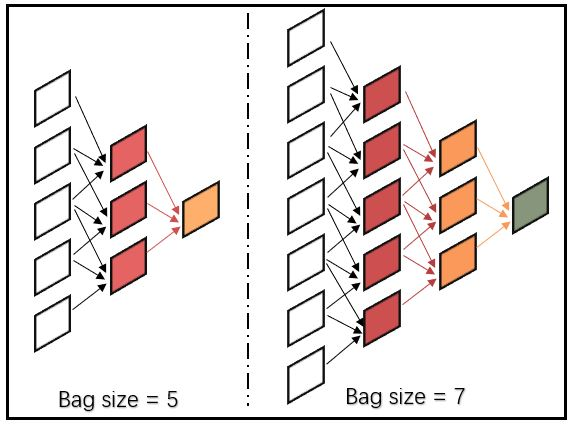
\includegraphics[width=1.0\linewidth]{agg_process.JPG}
\end{center}
  \caption{Two examples of Feature aggregation proceses}
\label{fig:long}
\label{fig:onecol}
\end{figure}


%%%%%%%%%%%%%%%%%%%%%%%%%%%% 4, Experiments %%%%%%%%%%%%%%%%%%%%%%%%%%%%%%%%%%%%
\section{Experiments}
In the experimental section, we trained and tested our model on two datasets, the human protein atlas datasets and the drosophila embryo datasets. On the human protein atlas datasets, we compared our method with the single-instance method without feature aggregation and the method of feature aggregation with simple averaging. At the same time, we also compared it wiht existing papers related to feature aggregation, such as MVCNN and NAN. Since the data of 3D objects is used in the paper of MVCNN, and the face dataset is used in NAN, which is different from the dataset in this experiment, So we retrained and tested them on the hap dataset based on their open source code. On the drosophila genetic dataset, we compared our experimental results with the result of the flyit paper. Since we use the same dataset, we directly compared the experimental results without unnecessary retraining and testing.


% 第五个图: hpa图片数据展示
\begin{figure}[t]
\begin{center}
% \fbox{\rule{0pt}{2in} \rule{0.9\linewidth}{0pt}}
  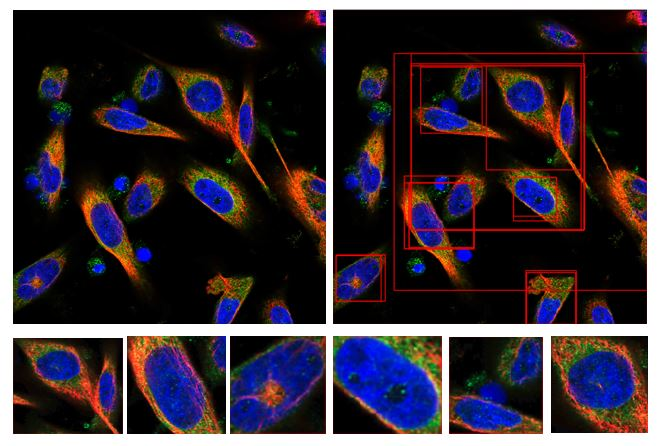
\includegraphics[width=0.9\linewidth]{figure6.JPG}
\end{center}
  \caption{Human protein atlas image has size of 2048 * 2048, and each image contained numerous identical organelles(top left).We use selective search algorithm to pick out the organelle in the original image(top right), and the captured iamges are shown in the bottom.  }
\label{fig:long}
\label{fig:onecol}
\end{figure}


%%%%%%%%%%% 4.1, Hpa Experiments %%%%%%%%%%%%%%%%%%%%
\subsection{Hpa experiment}

%%%%%% 4.1.1, Dataset introduction %%%%%%
\subsubsection{Dataset introduction}
The human protein dataset is derived from the human protein atlas database, which is designed to leverage various omics techniques(including antibody imaging, mass spectrometry, proteomics, etc) to map the expression and spatial distribution of all human proteins in cells and tissues. The database is free to use and aim to help speed up life science research and drug discovery. We crawled about 1600 packages from this database, each containing a different number of protein images. Each package represents a sample of multiple instances, and the category labels of all images in each package are consistent.

%%%%%% 4.1.2, Data pre-process %%%%%%
\subsubsection{Data pre-process}
In the above dataset, as shown in figure 5, the size of each image ranged from 800*800, 1728*1728 to 2048*2048, and each image contained numerous identical organelles. If such an image is directly input into the network model, we will face the problem that the number of data samples is not enough and the model is easy to over-fit. At the same time, because the data dimension is large, it will bring a huge amount of computation and heavy load to the training phase of the network. So, in this case, we use a selective search algorithm to pick out each organelle in the image for each image that we get. As shown in figure 5, the selective search algorithm selected most organelles in the cell. After that, we intercepted the candidate region coordinates provided by the selective search algorithm from the original image and resize it into a fixed size of 512*512. We use the captured image containing a single organelle as the image used in training to generate a new dataset. Some of the captured images are shown in figure 5.

%%%%%%%%%%%%%%%%%%%%%%%%%%%%%% 4.13, Experimental Setting %%%%%%%%%%%%%%%%%%%%%%%%
\subsubsection{Experimental Setting}
When training the model, we used the pytorch framework, and the hardware environment we used was 2.4GHz CPU, 32GB RAM, and two 2080Ti graphics cards. When optimizing the network, we adopted Adam optimizer\cite{ref25}, we set the learning rate of the network, $\beta_1$,$\beta_2$ to 0.0001, 0.9 and default value respectively. The batch size of the network is set as 16. In this experiment, the loss function we adopted is the stanard bce loss. The selected feature extraction network is resnet50 model, and the final classification number is 10 categories.To evaluate the performance of the model and compare it with previous research results, we used 4 generic multi-label classification metrics, namely AUC value, marco precision value, marco recall value, marco f1 value and micro f1 value.

%%%%%%%%%%%%%%%%%% 4.1.4, Result and analysis %%%%%%%%%%%%%%%%%%
\subsubsection{Result and analysis}
In the experiment of hpa dataset, we carried out two comparison experiments. The first comparison experiment compared our model with two baseline models. The first baseline model, which we called Single-Instace model, is denoted as SI, SI adpots the traditional Single-input-Single-output model for training.During the test, multiple instances are input for several times, and the predicted result is output at the maximum value. The second baseline model is called multi-instance model, which is denoted as $MI_{mean}$, $MI_{mean}$ adopts the same training mode of multi-input and single-output as DRAGN, except that $MI_{mean}$ adopts the simple method of averaging multiple features for feature aggregation. The experimental results are shown in table 1. As can be seen from table 1, the result of SI model is extremely poor when applied to the multiple instances. By comparing the results of $MI_{mean}$ and SI models, it can be seen that the experimental result can be greatly improved by adopting the feature aggregation of simple averaging formula. The last column in the table 1 is the result of DRAGN model, which achieved the best results on all metrics.

In the second set of comparative experiments, we compared the DRAGN model with the deep learning algorithms related to multiple instances aggregation. Here, we compared MVCNN, NAN, and SPoc\cite{ref28}, and the experimental results are shown in table 2. In the above deep learning algorithm, MVCNN takes the maximum value of multi-instance features to aggregate, NAN learned adaptive weights between multi-instance features by introducing an attention mechanism, SPoc used radial basis functions to aggregate each feature of multi-instance features. By introducing feature aggregation unit, DRAGN uses the newly proposed cyclic convolution for feature aggregation.As shown in table 2, the experimental results of DRAGN show great advantages in many metrics, and the performance in a few metrics are almost the same as the highest results.

%%%%%%%%%%%%% table 1 %%%%%%%%%%%%
\begin{table}
\normalsize
\begin{center}
\begin{tabular}{|c|c|c|c|c|c|}
\hline
Method & SI & $MI_{mean}$ & Ours \\
\hline\hline
AUC(\%) & 95.56 & 95.59  & \textbf{96.56} \\
macro precision(\%) & 65.45 & 86.67 & \textbf{90.13} \\
macro recall(\%) & 20.96 & 54.23 & \textbf{56.06} \\
macro F1(\%) & 27.95 & 62.56 & \textbf{65.15} \\
\hline
\end{tabular}
\end{center}
\caption{Comparison with the baseline model}
\end{table}

%%%%%%%%%%%%% table 2 %%%%%%%%%%%%
\begin{table}
\normalsize
\begin{center}
\begin{tabular}{|c|c|c|c|c|c|}
\hline
Method & MVCNN & NAN & SPoc & Ours \\
\hline\hline
AUC(\%) & 96.08 & 95.86 & 93.35 & \textbf{96.56} \\
macro precision(\%) & \textbf{91.58} & 81.43 & 79.21 & 90.13 \\
macro recall(\%) & 53.59 & 50.85 & 45.86 & \textbf{56.06}\\
macro F1(\%) & 62.75 & 58.18 & 54.72 & \textbf{65.15} \\
micro F1(\%) & \textbf{81.79} & 77.82 & 75.97 & \textbf{81.69} \\
sensitivity(\%) & 76.38 & 72.46 & 68.30 & \textbf{77.44} \\
specificity(\%) & \textbf{99.48} & 99.31 & 99.42 & \textbf{99.39} \\
\hline
\end{tabular}
\end{center}
\caption{Comparison with the deep learning model}
\end{table}

%%%%%%%%%%% 4.2, Drosophila embryo Experiments %%%%%%%%%%%%%%%%%%%%
\subsection{Drosophila embryo experiment}

%%%%%% 4.2.1, Dataset introduction %%%%%%
\subsubsection{Dataset introduction}
As a standard drosophila gene image data repository\cite{ref26}, flyexpress.net contains many standard drosophila gene image data. These iamge data were high-quality image data downloaded from BDGP, and they have been cut, aligned and scaled to a uniform size of 180*320. We crawled more than 4000 packages from the warehouse with about 10k images.The dataset is divided into train set, validation set and test set according to the ratio of 5:4:1.

%%%%%% 4.2.2, Data pre-process %%%%%%
\subsubsection{Data pre-process}
As a comparison experiment, we followed the same experimental setup as flyit's\cite{ref27} paper to conduct the same pre-processing for the crawled data.Specially, we also discarded the drosophila gene data of stage 1-3 containing only a small number of gene expression patterns, and only the top10 categories were selected for classification.

%%%%%% 4.2.3, Experimental Setting %%%%%%
\subsubsection{Experimental Setting}
As with the hpa dataset experiment, we use the pytorch framework to train the model. And the hardware environment we used was 2.4GHz CPU, 32GB RAM, and two 2080Ti graphics cards. When optimizing the network, we adopted Adam optimizer\cite{ref25}, we set the learning rate of the network, $\beta_1$,$\beta_2$ to 0.0001, 0.9 and default value respectively. The batch size of the network is set as 4. In this experiment, the loss function we adopted is the stanard bce loss. Due to the small amount of dataset, the lightweight network will be more advantageous. Therefore, the feature extraction module adopted here is resnet18 model, while the feature aggregation unit chooses L1Agg module. The final classification is 10 categories, and the selected evaluation metrics are the same as the flyit's\cite{ref27} metrics, namely AUC, macro f1 and micro f1.

%%%%%% 4.2.4, Result and analysis %%%%%%
\subsubsection{Result and analysis}

%%%%%%%%%%%%% table 3 %%%%%%%%%%%%
\begin{table}
\footnotesize
\begin{center}
\begin{tabular}{|c|c|c|c|c|c|}
\hline
Method & AUC(\%) & macro F1(\%)  & micro F1(\%)\\
\hline\hline
$ML_{LS}$ & 80.92 & 54.99 & 60.17 \\
$PMK_{SIFT}$ & 76.73 & 43.31 & 54.60 \\
$PMK_{comp}$ & 76.66 & 50.02 & 55.86 \\
$LR_{SOFT}$ & 82.95 & 57.72 & 62.28 \\
$PMK_{star}$ & 76.42 & 48.81 & 54.55 \\

$PMK_{clique}$ & 76.58 & 45.70 & 54.94 \\
$PML_{kcca}$ & 76.51 & 34.36 & 48.83 \\
$E-MIMLSVM^{+}$ & 84.60 & 59.80 & 64.00 \\
$HMIML$ & 85.30 & 63.98 & 66.73 \\
FlyIT & 93.59 & 71.81 & 71.08 \\ \hline 
$\textbf{Ours}$ & \textbf{94.77} & \textbf{74.74} & \textbf{74.79} \\
\hline
\end{tabular}
\end{center}
\caption{Comparison with the existing annotators and FlyIT}
\end{table}

The experimental results are shown in table 3, Here, we show all the relevant experimental results in the flyit paper in table3. At the same time, the experimental results of our model are also shown in the last row of table 3. As we can seen from table 3. As shown in the flyit paper, the flyit model has obvious advantages over other models, all of its metrics are generally higher than others. However, the metrics of our model are better than those of flyit. By comparing the result of the flyit model with those of DRAGN model in the last two lines of table 3, it can be seen that the model results of DRAGN exceed the result of flyit in all metrics, and there is a great improvement in macro F1 and micro F1 metrics. It can be seen from the above experimental results that, compared with the multi-instance stitching algorithm proposed by flyit, the feature aggregation algorithm proposed by DRAGN model has more advantages for the multi-instance problem.

\textbf{Qualitative visualization.} In order to explore what changes the DRAGN model will bring to the features, here, we use the drosophila dataset for a visual presentation before and after feature aggregation. The specific approach is as follows: first, we obtained the features of drosophila data using resnet model, and then use tsne algorithm to reduce the dimensionality of these features to a two-dimensional plane, the dimensionality reduction results are shown in figure 6. Then we use DRAGN model to aggregate the features just extracted, and then we also use tsne algorithm to reduce dimensions to a two-dimensional plane, and the dimensionality resuction results are shown in figure 7.By comparing figure 6 and figure 7, it can be seen that the features of different categories before aggregation have small margin and large overlap, which brings great difficulties to subsequent classifiers. After aggregation, features of different categories are relatively separated, with a large margin, which is convenient for subsequent classifiers to make accurate classification.

% 第6个图: 聚合前的分布
\begin{figure}[t]
\begin{center}
% \fbox{\rule{0pt}{2in} \rule{0.9\linewidth}{0pt}}
  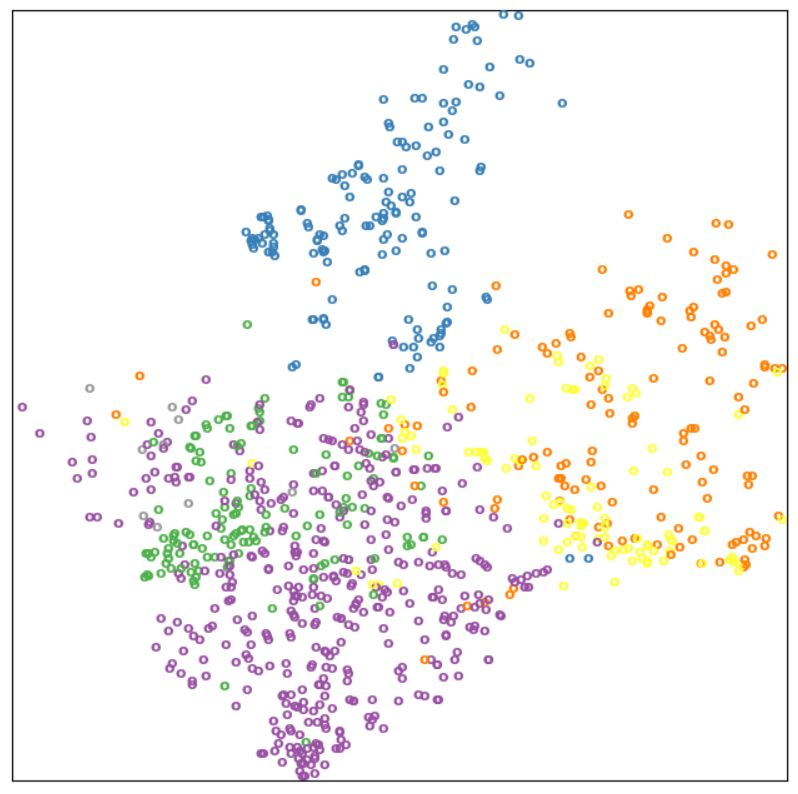
\includegraphics[width=0.9\linewidth]{original.JPG}
\end{center}
  \caption{the feature distribution before feature aggregation}
\label{fig:long}
\label{fig:onecol}
\end{figure}


% 第7个图: 聚合后的分布
\begin{figure}[t]
\begin{center}
% \fbox{\rule{0pt}{2in} \rule{0.9\linewidth}{0pt}}
  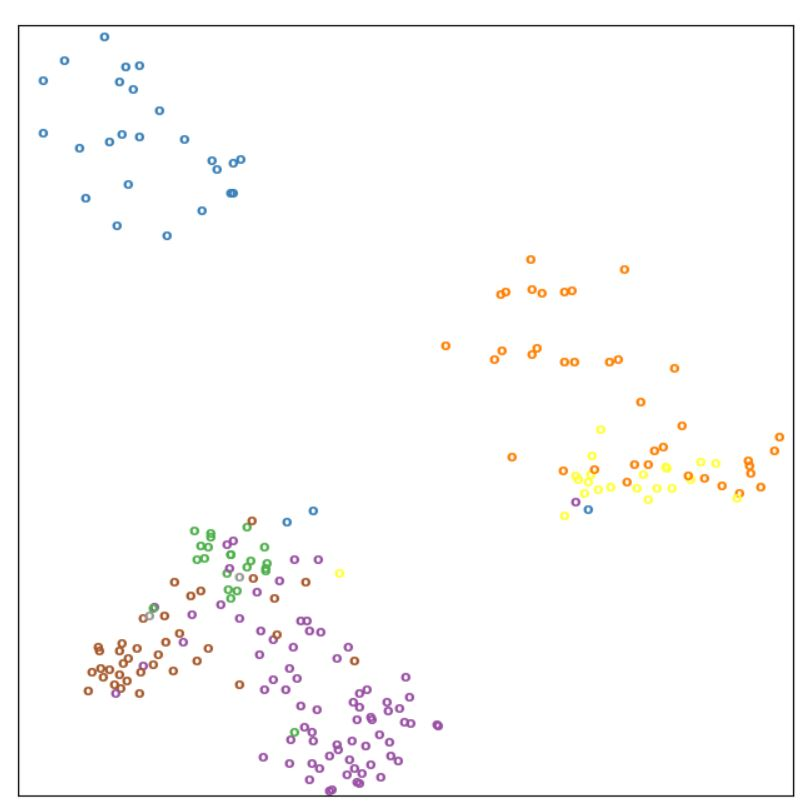
\includegraphics[width=0.9\linewidth]{agg.JPG}
\end{center}
    \caption{the feature distribution after feature aggregation}
\label{fig:long}
\label{fig:onecol}
\end{figure}


% 第8个图: 可视化权重
\begin{figure*}
\begin{center}
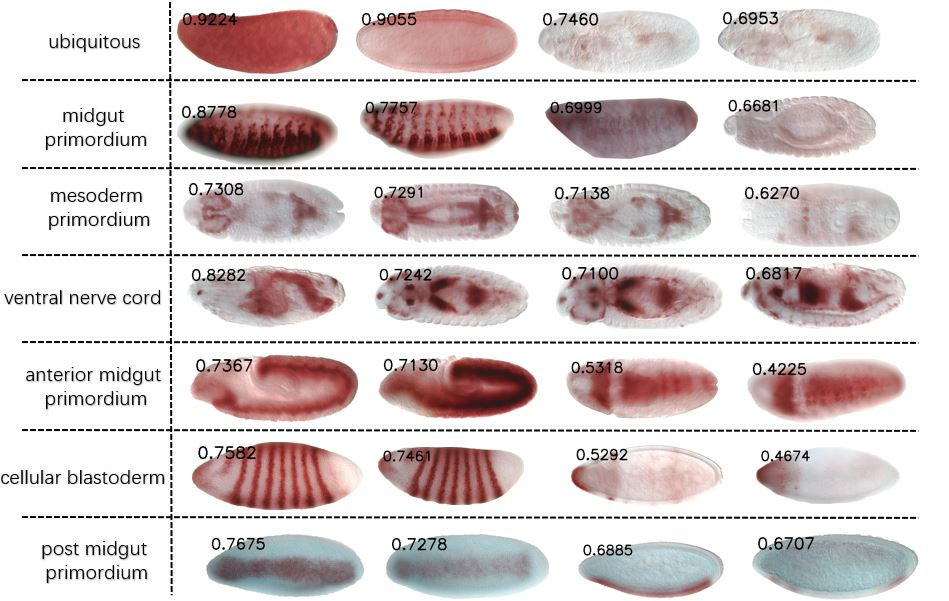
\includegraphics[width=0.8\linewidth]{flycompare.JPG}
\end{center}
   \caption{The weight distribution between the aggregated feature and the original images.}
\label{fig:short}
\end{figure*}

\textbf{Visualize feature similarity.} In many feature aggregation model, the attention mechanism is introduced. These models learn the weight of multiple images through the attention mechanism, and then use these weights to combine the aggregated output. In our model, although we do not have an explicit attention mechanism, our output features will also focus on input features which have more information through our feature aggregation algorithm, thus making our model have an implicit attention mechanism. To prove this opinion, we conduct the following experiments, first, we use DRAGN to obtain the features before and after aggregation, then calculate the cosine similarity of the aggregated feature and the input feature, and take the cosine similarity as the score value of the input images, and then sort the score values in descending order to get figure 9. As we can seen from figure 9, the aggregated feature is more similar to the features whose images have more information, but less similar to the features whose images have less effective information. This means that the features aggregated by DRGAN will automatically focus on the important features, that is, our model have an implicit attention mechanism.

%-------------------------------------------------------------------------

%%%%%%%%%%%%%%%%%%%%%%%%%%%% 5, Conclusion and Discussion %%%%%%%%%%%%%%%%%%%%%%%%%%%%%%%%%%%%
\section{Conclusion and Discussion}
This paper proposes a general network framework DRAGN for feature aggregation, which uses pre-trained resenet model for feature extraction, uses a newly designed feature aggregation module for feature aggregation, and applies the features after aggregation to downstream tasks. In this paper, the performance of DRAGN network is also tested on the hpa dataset and droophila gene dataset, and the experimental results are compared with the existing feature aggregation algorithm.The experimental results prove the advantages of DRAGN model.

Although our model has shown excellent performance in both of these two tasks, but the scope of our model is not limited to these two tasks. The DRAGN we proposed is a general feature aggregation network, we can easily change its components to make it suitable for other tasks and improve their performance.For example, in terms of feature extraction network, in addition to resnet series, we can also select other pre-trained network model, such as vgg series, Densenet, SENet, SEResnet and so on. After selecting the feature extraction network, we can also flexibly choose which layers of activation output to used as the extracted feature. Obviously, feature in the first layers of the network will be more textured and the feature in the last few layers of the network will be more semantic. The selection of different layers will have different influences on the final result of the model, it is even possible to select different layers at the same time and output them as features. It is also worth paying attention to the selection of different feature aggregation units, in this paper, we proposed three feature aggregation units with different complexity. When using our model framework, we can choose the appropriate feature aggregation unit according to the specific situation. In addition, although all experiments in this paper are based on post-aggregation, per-aggregation is also a worthwhile aggregation method.

%%%%%%%%%%%%%%%%%%%%%%%%%%%% 6, Future Work %%%%%%%%%%%%%%%%%%%%%%%%%%%%%%%%%%%%
\section{Future Work}
Although the experiments in this paper are carried out based on images from the biological field, our model is a general framework and not only confined to the biological field. As we described in the introduction, there are also scenes using feature aggregation in the field of natural images.Therefore, in the feature, we will consider applying DRAGN proposed in this paper to the field of natural images in order to improve the performance of related tasks.

In the future, we will also explore to use the our model to the field of biological sequences. Since most biological sequences domains have temporal information, we will consider to use RNN to design the feature aggregation units to capture temporal information between multiple features in the biological sequence domain. In this way, multiple biological sequences features can be effectively integrated to improve the metrics and performance of related tasks in the field of biological sequence.

%%%%%%%%%%%%%%%%%%%%%%%%%%%% 7, reference %%%%%%%%%%%%%%%%%%%%%%%%%%%%%%%%%%%%
{\small
\bibliographystyle{ieee_fullname}
\bibliography{egbib}
}

\end{document}
